\newpage
\subsection{Vermessungsaufgaben}


\hfill \break
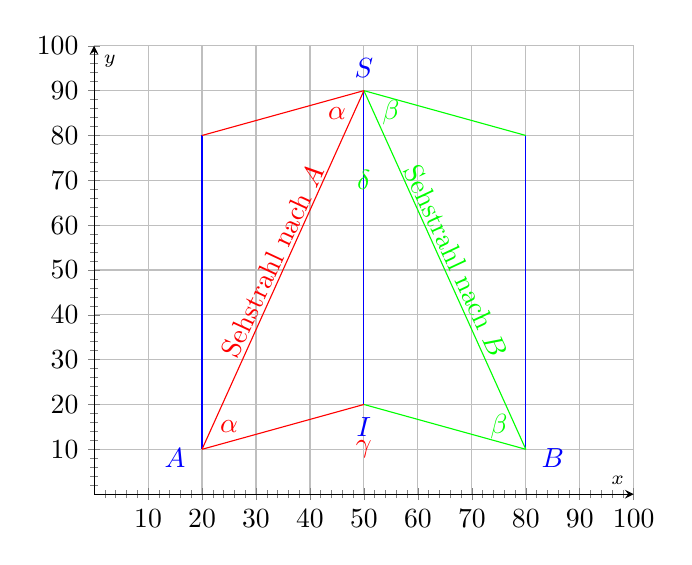
\begin{tikzpicture}[scale=1]
    \begin{axis}%
        [
            grid=major,
            xtick={0,10,...,100},
            minor x tick num=4,
            xmin=0,
            xmax=100,
            xlabel={\scriptsize $x$},
            axis x line=middle,
            ytick={0,10,...,100},
            minor y tick num=4,
            ymin=0,
            ymax=100,
            ylabel={\scriptsize $y$},
            axis y line=middle,
            no markers,
            samples=100,
            domain=-1:10,
        ]

        \draw[color=blue] (50,20) -- (50,90);
        \draw[color=blue] (20,10) -- (20,80);
        \draw[color=blue] (80,10) -- (80,80);
        \draw[color=green] (80,80) -- (50,90);
        \draw[color=green] (80,10) -- (50,20);
        \draw[color=green] (80,10) -- (50,90);
        \draw[color=red] (20,80) -- (50,90);
        \draw[color=red] (20,10) -- (50,20);
        \draw[color=red] (20,10) -- (50,90);

        \node[color=green,rotate=-65] at (67,52) {Sehstrahl nach $B$};
        \node[color=red,rotate=65] at (33,52) {Sehstrahl nach $A$};

        \node[color=red] at (25,15) {$\alpha$};
        \node[color=green] at (75,15) {$\beta$};
        \node[color=red] at (45,85) {$\alpha$};
        \node[color=green] at (55,85) {$\beta$};

        \node[color=red] at (50,10) {$\gamma$};
        \node[color=green] at (50,70) {$\delta$};
        \node[color=blue] at (15,8) {$A$};
        \node[color=blue] at (85,8) {$B$};
        \node[color=blue] at (50,95) {$S$};
        \node[color=blue] at (50,15) {$I$};


    \end{axis}
\end{tikzpicture}


\hfill \break
\begin{itemize}
    \item $\textcolor{red}{\alpha},\textcolor{green}{\beta} \rightarrow$ Hähenwinkel, von der Horizontale aus nach oben gemessen.
    \item $\textcolor{red}{\alpha},\textcolor{green}{\beta} \rightarrow$ Tiefenwinkel, von der Horizontale aus nach unten gemessen.
    \item $\textcolor{red}{\gamma}... Horizontalwinkel$ zwischen den 2 gedachten Linien.
    \item $\textcolor{green}{\delta}... Sehwinkel$ von 2 Sehstralen.
\end{itemize}

\newpage
\subsubsection{Beispiel 1: Der Fluss}

\hfill \break
Berechne die Breite eines Flusses, wenn in einem geradlinigen Uferstück die Standlinie AB (150m) abgesteckt wird
sowie die Winkel CAB (63°22') und CBA (44°30') zu einem am gegenüberliegenden Ufer liegenden Punkt C gemessen
wird.
(Lösung: 98,75m)

\hfill \break
\begin{itemize}
    \item Winkel $CAB = \alpha = 63.37$°
    \item Winkel $CBA = \beta = 44.5$°
    \item Winkel $BC = \gamma = 72.13$°
\end{itemize}

\hfill \break
Rechenweg:\\
\fboxrule=0.8pt \fcolorbox{black}{lightgray}{%
    \begin{tabular}[t]{@{}l@{}}
        $x = \frac{Sin(44.5)*150}{Sin(72.13)}$ \\
        $x = 110.47$                           \\
        \\
        $b=Sin(\alpha)/x$                      \\
        $b=Sin(63.37)*110.47$                  \\
        $b=98.75m$                              \\
    \end{tabular}}

\hfill \break
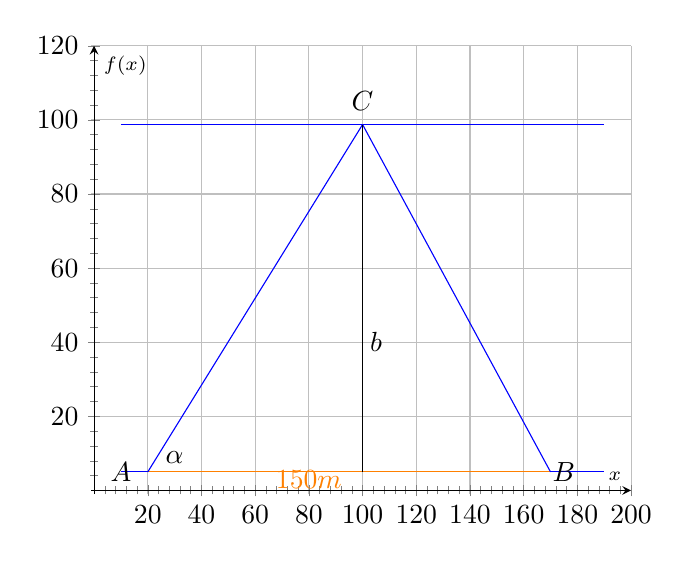
\begin{tikzpicture}[scale=1]
    \begin{axis}%
        [
            grid=major,
            xtick={0,20,...,200},
            minor x tick num=4,
            xmin=-1,
            xmax=200,
            xlabel={\scriptsize $x$},
            axis x line=middle,
            ytick={0,20,...,120},
            minor y tick num=4,
            ymin=-1,
            ymax=120,
            ylabel={\scriptsize $f(x)$},
            axis y line=middle,
            no markers,
            samples=100,
            domain=-1:10,
        ]

        \draw[color=blue] (10,5) -- (190,5);
        \draw[color=orange] (20,5) -- (170,5);
        \draw[color=blue] (10,98.75) -- (190,98.75);
        \draw[color=blue] (100,98.75) -- (20,5);
        \draw[color=blue] (100,98.75) -- (170,5);
        \draw[color=black] (100,98.75) -- (100,5);

        \node[color=black] at (10,5) {$A$};
        \node[color=black] at (175,5) {$B$};
        \node[color=black] at (100,105) {$C$};
        \node[color=black] at (105,40) {$b$};
        \node[color=black] at (30,9) {$\alpha$};
        \node[color=orange] at (80,3) {$150m$};
    \end{axis}
\end{tikzpicture}
\newpage
\subsubsection{Beispiel 2: Der Antennemast}

\hfill \break
Der Antennenmast eines Fernsehturms hat die Höhe h = 75m. Von einem Geländepunkt P werden Spitze und Fußpunkt
des Antennenmast unter den Höhenwinkeln a = 24°12' und ß = 17°42' gesehen. Ermittle die Höhe des Fernsehturms
mit Sendemast.
(Lösung: 258,73m)

\hfill \break
\begin{itemize}
    \item Winkel $\alpha = 24.2$°
    \item Winkel $\beta = 17+\frac{42}{60}$°
    \item Winkel $\gamma = 24.2-1.7=6.5$°
    \item Winkel $\delta = 180 - 90 - 17.7 = 72.3$°
    \item Winkel $\epsilon = 107.7$°
    \item Winkel $\zeta = 65.8$°
\end{itemize}

\hfill \break
Rechenweg:\\
\fboxrule=0.8pt \fcolorbox{black}{lightgray}{%
    \begin{tabular}[t]{@{}l@{}}
        $\frac{75}{Sin(\alpha)} = \frac{\gamma}{Sin(\zeta)}$ \\
        $\frac{75}{Sin(\alpha)} = \gamma$                    \\
        $y = 604.3$                                          \\
        \\
        $Sin(\beta) = \frac{x}{y}$                           \\
        $Sin(\beta)*\gamma = x$                              \\
        $x = 183.73$                                         \\
        \\
        $H = 183.73 + 75 = 258.73$                           \\
    \end{tabular}}

%//TODO add drawing